% Use only LaTeX2e, calling the article.cls class and 12-point type.

\documentclass[12pt]{article}

\usepackage{caption}
\usepackage{subcaption}

% Users of the {thebibliography} environment or BibTeX should use the
% scicite.sty package, downloadable from *Science* at
% www.sciencemag.org/about/authors/prep/TeX_help/ .
% This package should properly format in-text
% reference calls and reference-list numbers.

\usepackage{scicite}
\usepackage[pdftex]{graphicx}
\usepackage{amsthm}
\usepackage{mathtools}
\usepackage[utf8]{inputenc}
\usepackage[T1]{fontenc}
% Use times if you have the font installed; otherwise, comment out the
% following line.

\usepackage{times}

% The preamble here sets up a lot of new/revised commands and
% environments.  It's annoying, but please do *not* try to strip these
% out into a separate .sty file (which could lead to the loss of some
% information when we convert the file to other formats).  Instead, keep
% them in the preamble of your main LaTeX source file.
\usepackage[utf8]{inputenc}


% The following parameters seem to provide a reasonable page setup.

\topmargin 0.0cm
\oddsidemargin 0.2cm
\textwidth 16cm 
\textheight 21cm
\footskip 1.0cm


%The next command sets up an environment for the abstract to your paper.

\newenvironment{sciabstract}{%
\begin{quote} \bf}
{\end{quote}}


% If your reference list includes text notes as well as references,
% include the following line; otherwise, comment it out.

\renewcommand\refname{Referências e Notas}

% The following lines set up an environment for the last note in the
% reference list, which commonly includes acknowledgments of funding,
% help, etc.  It's intended for users of BibTeX or the {thebibliography}
% environment.  Users who are hand-coding their references at the end
% using a list environment such as {enumerate} can simply add another
% item at the end, and it will be numbered automatically.

\newcounter{lastnote}
\newenvironment{scilastnote}{%
\setcounter{lastnote}{\value{enumiv}}%
\addtocounter{lastnote}{+1}%
\begin{list}%
{\arabic{lastnote}.}
{\setlength{\leftmargin}{.22in}}
{\setlength{\labelsep}{.5em}}}
{\end{list}}


% Include your paper's title here

\title{Aplicação de {\it Simulated Anealing\/} Para o Problema de Corte 2D Guilhotinado}

% Place the author information here.  Please hand-code the contact
% information and notecalls; do *not* use \footnote commands.  Let the
% author contact information appear immediately below the author names
% as shown.  We would also prefer that you don't change the type-size
% settings shown here.

\author
{Aeliton G. Silva,$^{1}$ Alano Martins,$^{1}$\\
\\
\normalsize{$^{1}$Mestrado Academico em Ciência da Computação, Universidade Estadual do Ceará,}\\
\normalsize{Av. Dr. Silas Munguba, 1700, Campus do Itaperi, Fortaleza-CE, Brasil}\\
\\
%\normalsize{$^\ast$To whom correspondence should be addressed; E-mail:  jsmith@wherever.edu.}
}

% Include the date command, but leave its argument blank.

\date{}



%%%%%%%%%%%%%%%%% END OF PREAMBLE %%%%%%%%%%%%%%%%



\begin{document} 

% Double-space the manuscript.

\baselineskip24pt

% Make the title.

\maketitle 



% Place your abstract within the special {sciabstract} environment.

\begin{sciabstract}
    Este documento apresenta a aplicação da metaheurística \textit{Simulated
    Anealing} ao problema de Corte Bidmensional Guilhotinado. Provemos os
    resultados da execução de 10 instâncias, cada uma executada 3 vezes e
    selecionada a melhor delas para apresentação em uma tabela com todos os
    melhores resultados obtidos. Apresentamos também os métodos mais
    importantes da implementação, em python, de nossa solução.
\end{sciabstract}

% In setting up this template for *Science* papers, we've used both
% the \section* command and the \paragraph* command for topical
% divisions.  Which you use will of course depend on the type of paper
% you're writing.  Review Articles tend to have displayed headings, for
% which \section* is more appropriate; Research Articles, when they have
% formal topical divisions at all, tend to signal them with bold text
% that runs into the paragraph, for which \paragraph* is the right
% choice.  Either way, use the asterisk (*) modifier, as shown, to
% suppress numbering.

\section*{Introdução}

O corte guilhotinado 2D para objetos retangulares é um desafio para otimização do aproveitamento dessas peças, reduzindo-as em objetos menores com o maior aproveitamento, ou seja, menor perda de materiais restantes após os cortes. 
Apesar do facil entendimento da problemática, o corte guilhotinável 2D é considerado um problema \textit{NP-HARD}, o qual não há algoritmos deterministicos para resolução em tempo hábil para instâncias de médio ou grande porte.
Esse problema é dado por uma grande variedade de arranjos possíveis, tornando inviável uso de métodos exatos. Assim os métodos heuristicos e meta heuristicos são uma boa solução.
Esse trabalho visa demonstrar uma implementação para o problema de corte guilhotinado 2D utilizando a meta heuristica \textit{Simulated Annealing}. 

\section*{Definições}
	
	Diversos processos produtivos passam por uma atividade de corte em diversos tipos de materiais, afim de reduzir uma peça maior em várias outras menores com a finalidade de atender demanda por itens especificos, porém reduzindo os disperdicios do material original. 
	Se um corte numa área retangular resulta em outros dois retangulos, esse problema é considerado guilhotinável ortogonal e quando isso não ocorre, guilhotinável não ortogonal. Para restringir o problema, os cortes devem ser realizados paralelos ao lado dos retângulos como demonstrado na figura:
	
	\begin{figure}[h]
    \centering
    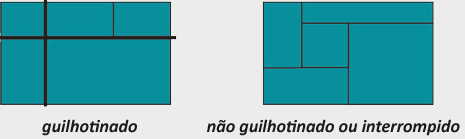
\includegraphics[width=15cm, height=5cm]{imagens/guilhotine}
    \caption{Exemplos de cortes}
  \end{figure}
	
	O problema abordado nesse trabalho é para cortes em peças limitadas pelo tamanho do objeto origianal e maior, realizando apenas cortes guilhotináveis e não estagiados, esse problema também é conhecido como  Problema de Corte Bidimensional Guilhotinado e Restrito.
	

\section*{Perturbação e Vizinhança}

Following are a few things to keep in mind in coding equations,
tables, and figures for submission to {\it Science}.

\paragraph*{In-line math.}  The utility that we use for converting
from \LaTeX\ to HTML handles in-line math relatively well.  It is best
to avoid using built-up fractions in in-line equations, and going for
the more boring ``slash'' presentation whenever possible --- that is,
for \verb+$a/b$+ (which comes out as $a/b$) rather than
\verb+$\frac{a}{b}$+ (which compiles as $\frac{a}{b}$).  Likewise,
HTML isn't tooled to handle certain overaccented special characters
in-line; for $\hat{\alpha}$ (coded \verb+$\hat{\alpha}$+), for
example, the HTML translation code will return [\^{}$(\alpha)$].
Don't drive yourself crazy --- but if it's possible to avoid such
constructs, please do so.  Please do not code arrays or matrices as
in-line math; display them instead.  And please keep your coding as
\TeX-y as possible --- avoid using specialized math macro packages
like \texttt{amstex.sty}.

\paragraph*{Displayed math.} Our HTML converter sets up \TeX\
displayed equations using nested HTML tables.  That works well for an
HTML presentation, but Word chokes when it comes across a nested
table in an HTML file.  We surmount that problem by simply cutting the
displayed equations out of the HTML before it's imported into Word,
and then replacing them in the Word document using either images or
equations generated by a Word equation editor.  Strictly speaking,
this procedure doesn't bear on how you should prepare your manuscript
--- although, for reasons best consigned to a note \cite{nattex}, we'd
prefer that you use native \TeX\ commands within displayed-math
environments, rather than \LaTeX\ sub-environments.

\paragraph*{Tables.}  The HTML converter that we use seems to handle
reasonably well simple tables generated using the \LaTeX\
\texttt{\{tabular\}} environment.  For very complicated tables, you
may want to consider generating them in a word processing program and
including them as a separate file.

\paragraph*{Figures.}  Figure callouts within the text should not be
in the form of \LaTeX\ references, but should simply be typed in ---
that is, \verb+(Fig. 1)+ rather than \verb+\ref{fig1}+.  For the
figures themselves, treatment can differ depending on whether the
manuscript is an initial submission or a final revision for acceptance
and publication.  For an initial submission and review copy, you can
use the \LaTeX\ \verb+{figure}+ environment and the
\verb+\includegraphics+ command to include your PostScript figures at
the end of the compiled PostScript file.  For the final revision,
however, the \verb+{figure}+ environment should {\it not\/} be used;
instead, the figure captions themselves should be typed in as regular
text at the end of the source file (an example is included here), and
the figures should be uploaded separately according to the Art
Department's instructions.


\section*{Meta-Heurística \textit{Simulated Anealing}}

A meta heuristica Simulated Annealing (S.A) é uma técnica oriunda de uma analogia com a termodinamica para obter estados de baixas energias em um sólido. Como meta heuristica, ela é utilizada em problemas de otimização de busca local com probabilidade. 
Inicialmente o S.A a busca a partir de um indice qualquer, iniciando um laço em que cada interação procura um candidato seguinte para um ponto minimo na vinzinhança do atual candidato. Essa forma é dada pela seguinte diferença entre as funções objetivas:

$ {\triangle = f (sˆ1) - f(s) }$

Logo se $ {\triangle < 0 }$, houve uma diminuição na função objetiva e $ sˆ1$ é considerava como nova solução. Caso $ {\triangle = 0 }$ ou $ {\triangle > 0 }$ houve um aumento ou estabilidade da energia e a aceitação dessa solução será feita sobre um fator estatistico onde é mais provável para autas temperaturas e menos provável para menores. O fator utilizado é conhecido como fator de Boltzmann, dado por: $ {e^{(\triangle / T)} }$ onde T é a temperatura que regula a aceitação da solução de pior custo.

What you should send to {\it Science\/} will depend on the stage your manuscript is in:

\begin{itemize}
\item {\bf Important:} If you're sending in the initial submission of
  your manuscript (that is, the copy for evaluation and peer review),
  please send in {\it only\/} a PostScript or PDF version of the
  compiled file (including figures).  Please do not send in the \TeX\ 
  source, \texttt{.sty}, \texttt{.bbl}, or other associated files with
  your initial submission.  (For more information, please see the
  instructions at our Web submission site,
  http://www.submit2science.org/ .)
\item When the time comes for you to send in your revised final
  manuscript (i.e., after peer review), we require that you include
  all source files and generated files in your upload.  Thus, if the
  name of your main source document is \texttt{ltxfile.tex}, you
  need to include:
\begin{itemize}
\item \texttt{ltxfile.tex}.
\item \texttt{ltxfile.aux}, the auxilliary file generated by the
  compilation.
\item A PostScript file (compiled using \texttt{dvips} or some other
  driver) of the \texttt{.dvi} file generated from
  \texttt{ltxfile.tex}, or a PDF file distilled from that
  PostScript.  You do not need to include the actual \texttt{.dvi}
  file in your upload.
\item From B{\small{IB}}\TeX\ users, your bibliography (\texttt{.bib})
  file, {\it and\/} the generated file \texttt{ltxfile.bbl} created
  when you run B{\small{IB}}\TeX.
\item Any additional \texttt{.sty} and \texttt{.bst} files called by
  the source code (though, for reasons noted earlier, we {\it
    strongly\/} discourage the use of such files beyond those
  mentioned in this document).
\end{itemize}
\end{itemize}

% Your references go at the end of the main text, and before the
% figures.  For this document we've used BibTeX, the .bib file
% scibib.bib, and the .bst file Science.bst.  The package scicite.sty
% was included to format the reference numbers according to *Science*
% style.

\section*{Execução dos Testes}


\begin{figure}
\centering
\begin{subfigure}{.5\textwidth}
  \centering
  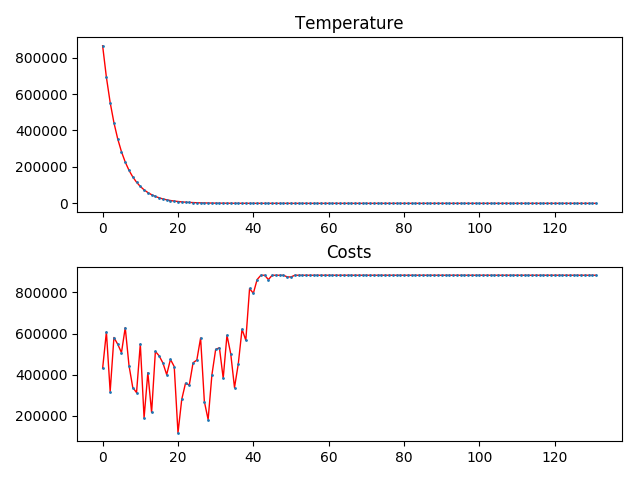
\includegraphics[width=1\linewidth]{results/cut12/3/plot}
  \label{fig:sub1}
\end{subfigure}%
\begin{subfigure}{.5\textwidth}
  \centering
  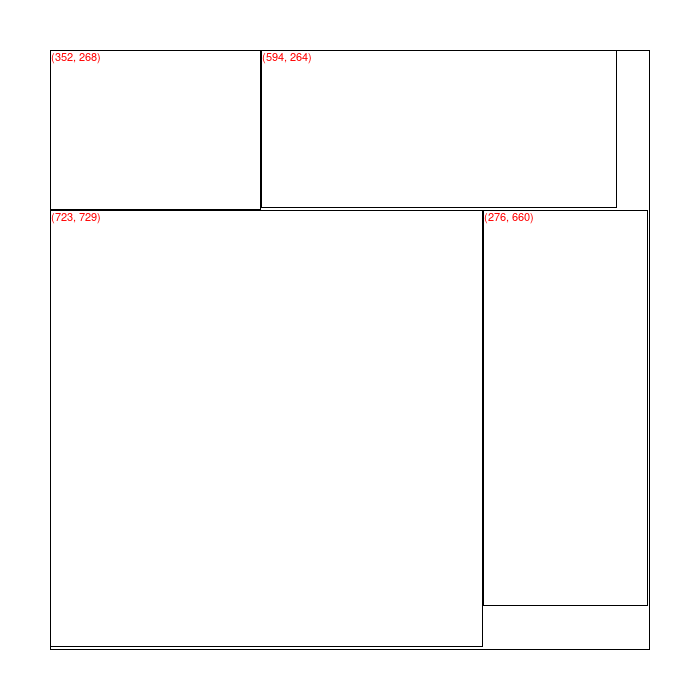
\includegraphics[width=1\linewidth]{results/cut12/3/cut}
  \label{fig:sub2}
\end{subfigure}
\caption{Instancia cut12.txt, Solução: 975059, desperdício de 2.49\% de 1000x1000, {(599, 269): 1, (359, 728): 1, (352, 268): 1, (640, 716): 1}}
\label{fig:test}
\end{figure}


\begin{figure}
\centering
\begin{subfigure}{.5\textwidth}
  \centering
  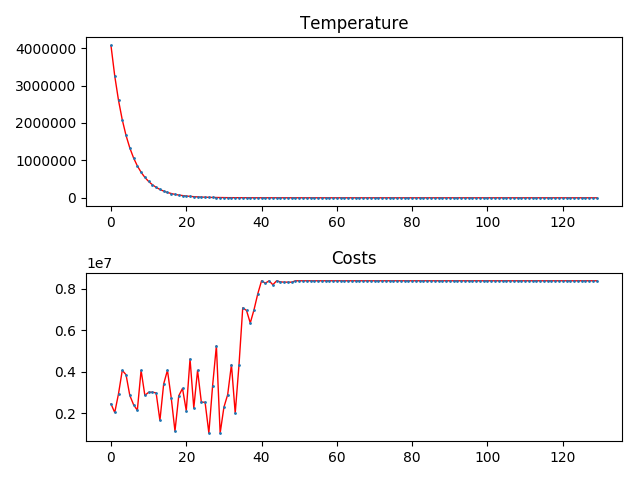
\includegraphics[width=1\linewidth]{results/cut13/1/plot}
  \label{fig:sub1}
\end{subfigure}%
\begin{subfigure}{.5\textwidth}
  \centering
  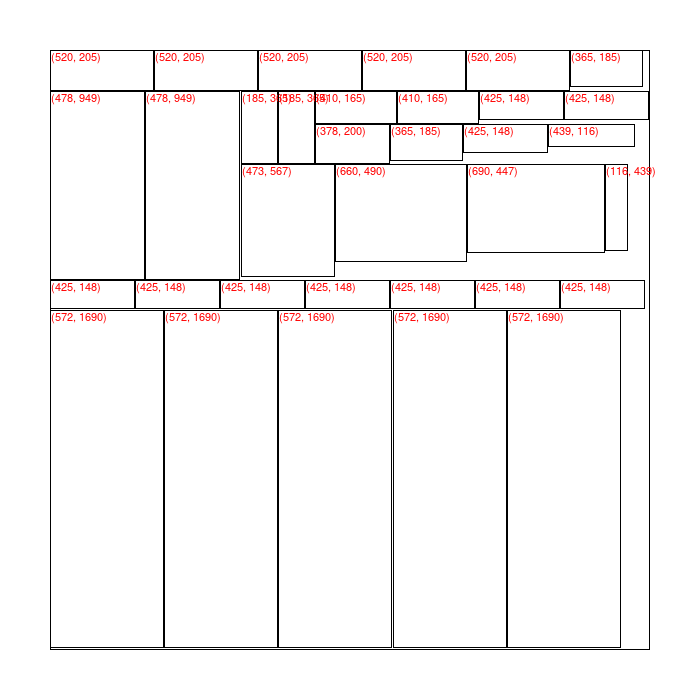
\includegraphics[width=1\linewidth]{results/cut13/1/cut}
  \label{fig:sub2}
\end{subfigure}
\caption{Instancia cut13.txt, Solução: 8212359, desperdício de 8.75\% de 3000x3000, {(540, 530): 1, (496, 555): 1, (520, 205): 1, (365, 185): 1, (116, 439): 1, (949, 445): 2, (296, 425): 1, (572, 1890): 5, (410, 165): 2, (148, 425): 1, (530, 540): 1, (205, 520): 1, (200, 378): 1, (567, 473): 1}}
\label{fig:test}
\end{figure}



\bibliography{scibib}

\bibliographystyle{Science}



% Following is a new environment, {scilastnote}, that's defined in the
% preamble and that allows authors to add a reference at the end of the
% list that's not signaled in the text; such references are used in
% *Science* for acknowledgments of funding, help, etc.

\begin{scilastnote}
\item We've included in the template file \texttt{scifile.tex} a new
environment, \texttt{\{scilastnote\}}, that generates a numbered final
citation without a corresponding signal in the text.  This environment
can be used to generate a final numbered reference containing
acknowledgments, sources of funding, and the like, per {\it Science\/}
style.
\end{scilastnote}




% For your review copy (i.e., the file you initially send in for
% evaluation), you can use the {figure} environment and the
% \includegraphics command to stream your figures into the text, placing
% all figures at the end.  For the final, revised manuscript for
% acceptance and production, however, PostScript or other graphics
% should not be streamed into your compliled file.  Instead, set
% captions as simple paragraphs (with a \noindent tag), setting them
% off from the rest of the text with a \clearpage as shown  below, and
% submit figures as separate files according to the Art Department's
% instructions.


\clearpage

\noindent {\bf Fig. 1.} Please do not use figure environments to set
up your figures in the final (post-peer-review) draft, do not include graphics in your
source code, and do not cite figures in the text using \LaTeX\
\verb+\ref+ commands.  Instead, simply refer to the figure numbers in
the text per {\it Science\/} style, and include the list of captions at
the end of the document, coded as ordinary paragraphs as shown in the
\texttt{scifile.tex} template file.  Your actual figure files should
be submitted separately.



\end{document}




















